\section{Augmented Unlinkable CC Protocol: Protecting against Malicious Retailers}
\label{sec:unlinkable-design-2}

This protocol is very similar to the Basic Unlinkable Protocol described in Section \ref{sec:unlinkable-design-1}.
In the Basic protocol, a 93-bit token was used to identify a customer to the Wallet Server.
In the Augmented protocol, the token consists of only 80 bits, leaving 13 bits left over to bind the price to the token.

When the Wallet Server receives a Registration message, it stores the card information and associates a card identifier \emph{ID} with this record.
It also generates a secret key \emph{secret} associated with this card.
In the Augmented protocol, the Wallet Server responds to the Registration message with this identifier \emph{ID} and the key \emph{D}.
The Wallet Application stores these values securely, associating them with the credit card being registered.
The protocol then operates as follows, and is illustrated in Figure \ref{fig:unlinkable-2}:

\begin{figure}[h!]
  \caption{Augmented Unlinkable CC Protocol}
  \centering
    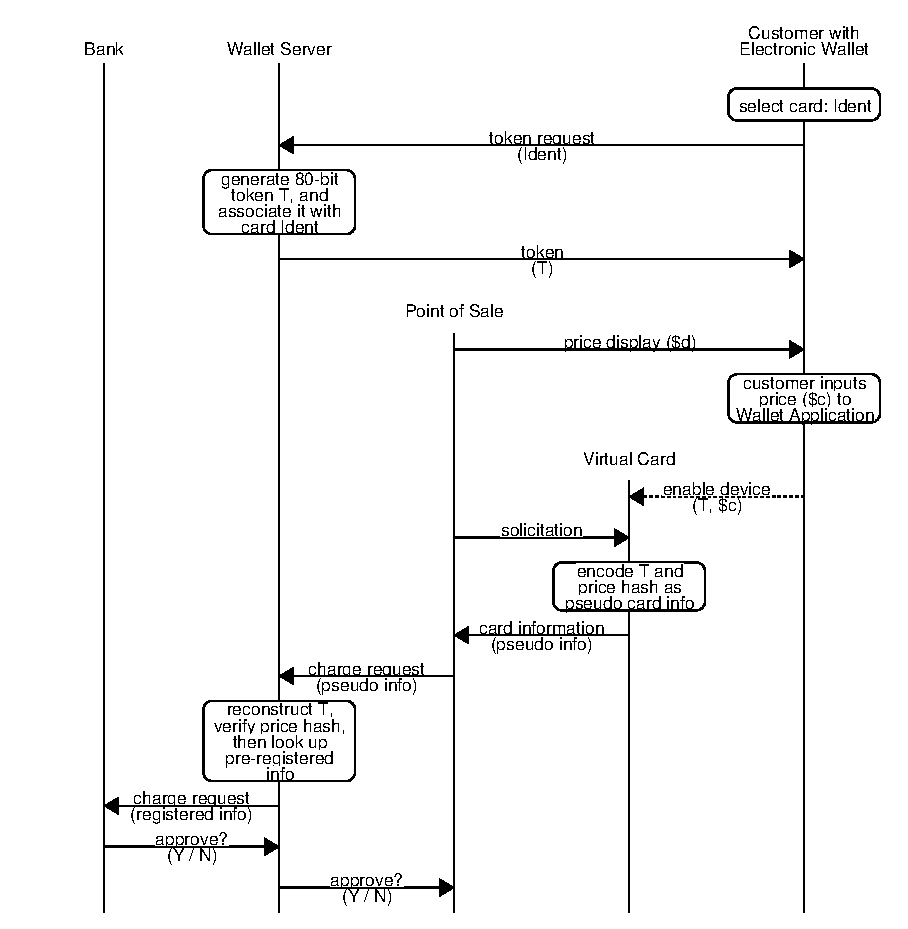
\includegraphics{img/unlinkable-2.eps}
  \label{fig:unlinkable-2}
\end{figure}

\begin{enumerate}
\item The customer selects a credit card in the Wallet Application.
\item The Wallet Application sends a Token Request message to the Wallet Server.
    This message consists of the card identifier \emph{ID} associated with the selected card, and is sent securely over the Internet.
    Note that this message must also be authenticated, to prevent a customer from requesting a token to a different customer's card.
\item The Wallet Server then generates a random 80-bit token \emph{T}, and associates it with card \emph{ID}.
    It responds to the Wallet Application with \emph{T}.
\item The Wallet Application now begins listening for Solicitation messages.
\item The point of sale displays the price to charge (\$d) on its screen.
\item The customer enters the price to be charged (\$c) into the Wallet Application.
\item The point of sale sends a Solicitation message to the Wallet Application over the NFC channel.
\item The Wallet Application looks up the 80-bit token \emph{T} which was issued for the card selected by the customer.
    It also calculates the hash of token \emph{T} combined with price \$c, keyed with key \emph{secret}, and selects the first 13 bits.
    It combines the 80-bit token with this 13-bit hash to acquire a 93-bit value.
    It then converts this value into a 28-digit number \emph{k}, and responds with an \emph{NFC} Card Information message as before.
\item The point of sale constructs an \emph{NFC} Charge Request message from the (pseudo) Card number, Expiration date, iCVV, and the price it wishes to charge.
    This message is sent to the bank named in the Card Information message.
    As a result, the Charge Request message is directed to the Wallet Server and \emph{not} an actual bank.
    Note that from the perspective of the point of sale, the Wallet Server appears to be a bank like any other.
\item The Wallet Server reconstructs \emph{k} from the Charge Request message, and computes the 80-bit token and 13-bit price hash that it represents.
    The Wallet Server then searches its database for the token, to identify the card used in this transaction.
    If no result is found, the Wallet Server sends a ``declined'' Acceptance message to the point of sale, and aborts the protocol.
    Otherwise, the secret key \emph{secret} is retrieved from the Wallet Server's database, and the Wallet Server calculates its own version of the price hash
        using the price issued in the Charge Request message.
    If the Wallet Server's price hash does not match the price hash in the Charge request, the Wallet Server sends a ``declined'' Acceptance message to the point of sale, and aborts the protocol.
    Otherwise, the stored card details are retrieved from the Wallet Server's database.
    The Wallet Server then invalidates token \emph{k}, and sends a \emph{visual} Charge Request to the card's bank with the following fields:
    \begin{itemize}
    \item Cardholder name
    \item Card number
    \item Expiration date
    \item Billing address
    \end{itemize}
    Note that unlike the Card Information message sent by the Wallet Application, this data reflects the actual credit card information.
\item The bank receives the \emph{visual} Charge Request from the Wallet Server,
    and processes this transaction as normal.
    Finally, it responds to the Wallet Server with an Acceptance message indicating whether the charge has been accepted.
\item The Wallet Server forwards the bank's Acceptance message to the point of sale.
\end{enumerate}